\documentclass{article}\usepackage[]{graphicx}\usepackage[]{color}
% maxwidth is the original width if it is less than linewidth
% otherwise use linewidth (to make sure the graphics do not exceed the margin)
\makeatletter
\def\maxwidth{ %
  \ifdim\Gin@nat@width>\linewidth
    \linewidth
  \else
    \Gin@nat@width
  \fi
}
\makeatother

\definecolor{fgcolor}{rgb}{0.345, 0.345, 0.345}
\newcommand{\hlnum}[1]{\textcolor[rgb]{0.686,0.059,0.569}{#1}}%
\newcommand{\hlstr}[1]{\textcolor[rgb]{0.192,0.494,0.8}{#1}}%
\newcommand{\hlcom}[1]{\textcolor[rgb]{0.678,0.584,0.686}{\textit{#1}}}%
\newcommand{\hlopt}[1]{\textcolor[rgb]{0,0,0}{#1}}%
\newcommand{\hlstd}[1]{\textcolor[rgb]{0.345,0.345,0.345}{#1}}%
\newcommand{\hlkwa}[1]{\textcolor[rgb]{0.161,0.373,0.58}{\textbf{#1}}}%
\newcommand{\hlkwb}[1]{\textcolor[rgb]{0.69,0.353,0.396}{#1}}%
\newcommand{\hlkwc}[1]{\textcolor[rgb]{0.333,0.667,0.333}{#1}}%
\newcommand{\hlkwd}[1]{\textcolor[rgb]{0.737,0.353,0.396}{\textbf{#1}}}%
\let\hlipl\hlkwb

\usepackage{framed}
\makeatletter
\newenvironment{kframe}{%
 \def\at@end@of@kframe{}%
 \ifinner\ifhmode%
  \def\at@end@of@kframe{\end{minipage}}%
  \begin{minipage}{\columnwidth}%
 \fi\fi%
 \def\FrameCommand##1{\hskip\@totalleftmargin \hskip-\fboxsep
 \colorbox{shadecolor}{##1}\hskip-\fboxsep
     % There is no \\@totalrightmargin, so:
     \hskip-\linewidth \hskip-\@totalleftmargin \hskip\columnwidth}%
 \MakeFramed {\advance\hsize-\width
   \@totalleftmargin\z@ \linewidth\hsize
   \@setminipage}}%
 {\par\unskip\endMakeFramed%
 \at@end@of@kframe}
\makeatother

\definecolor{shadecolor}{rgb}{.97, .97, .97}
\definecolor{messagecolor}{rgb}{0, 0, 0}
\definecolor{warningcolor}{rgb}{1, 0, 1}
\definecolor{errorcolor}{rgb}{1, 0, 0}
\newenvironment{knitrout}{}{} % an empty environment to be redefined in TeX

\usepackage{alltt} 
\usepackage{graphicx} 
%Title 
\title{PREVISION PARA ALMENDRICOS} 
\date{\today} 
\author{Meteored}
\IfFileExists{upquote.sty}{\usepackage{upquote}}{}
\begin{document} 
  
\maketitle % Create cover page 
%PREVISION PARA ALMENDRICOS 






Prediccion para Almendricos [Murcia;Espana]


NOTA: PRECIPITACION HORARIA PRIMERAS 24H!


\begin{figure}[h!]
\begin{knitrout}
\definecolor{shadecolor}{rgb}{0.969, 0.969, 0.969}\color{fgcolor}
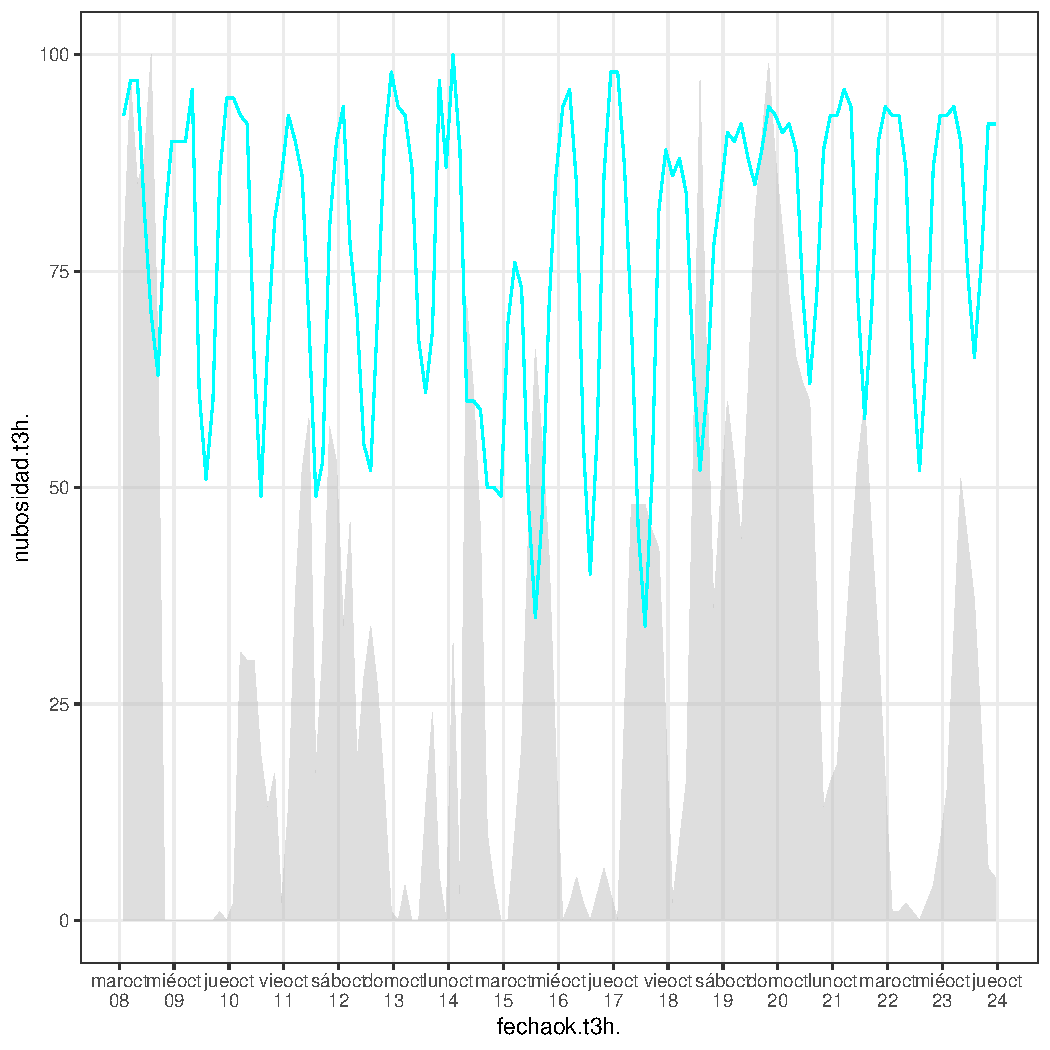
\includegraphics[width=\maxwidth]{figure/Figprec-1} 

\end{knitrout}
\end{figure}


\begin{figure}[h!]
\begin{knitrout}
\definecolor{shadecolor}{rgb}{0.969, 0.969, 0.969}\color{fgcolor}
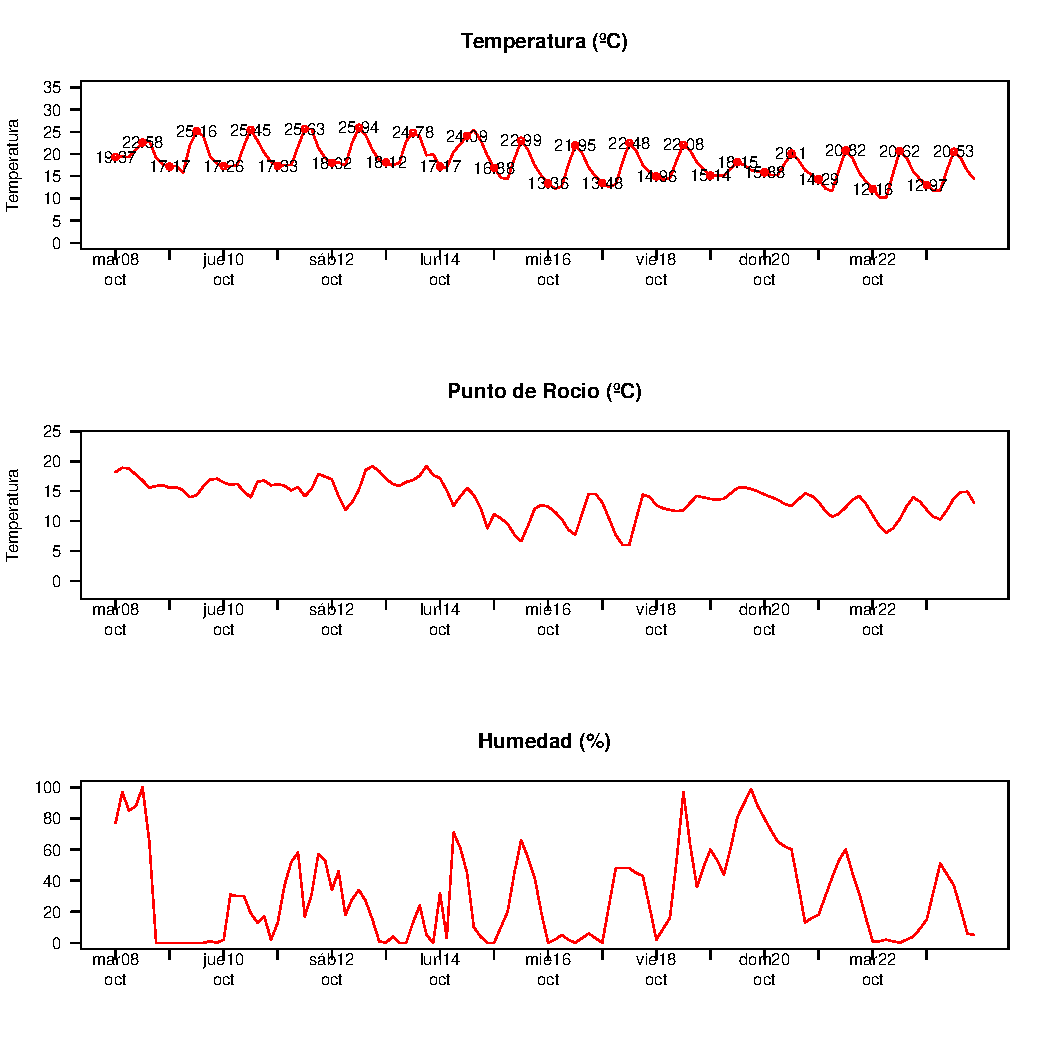
\includegraphics[width=\maxwidth]{figure/Figtemp-1} 

\end{knitrout}
\end{figure}

\begin{figure}[h!]
\begin{knitrout}
\definecolor{shadecolor}{rgb}{0.969, 0.969, 0.969}\color{fgcolor}
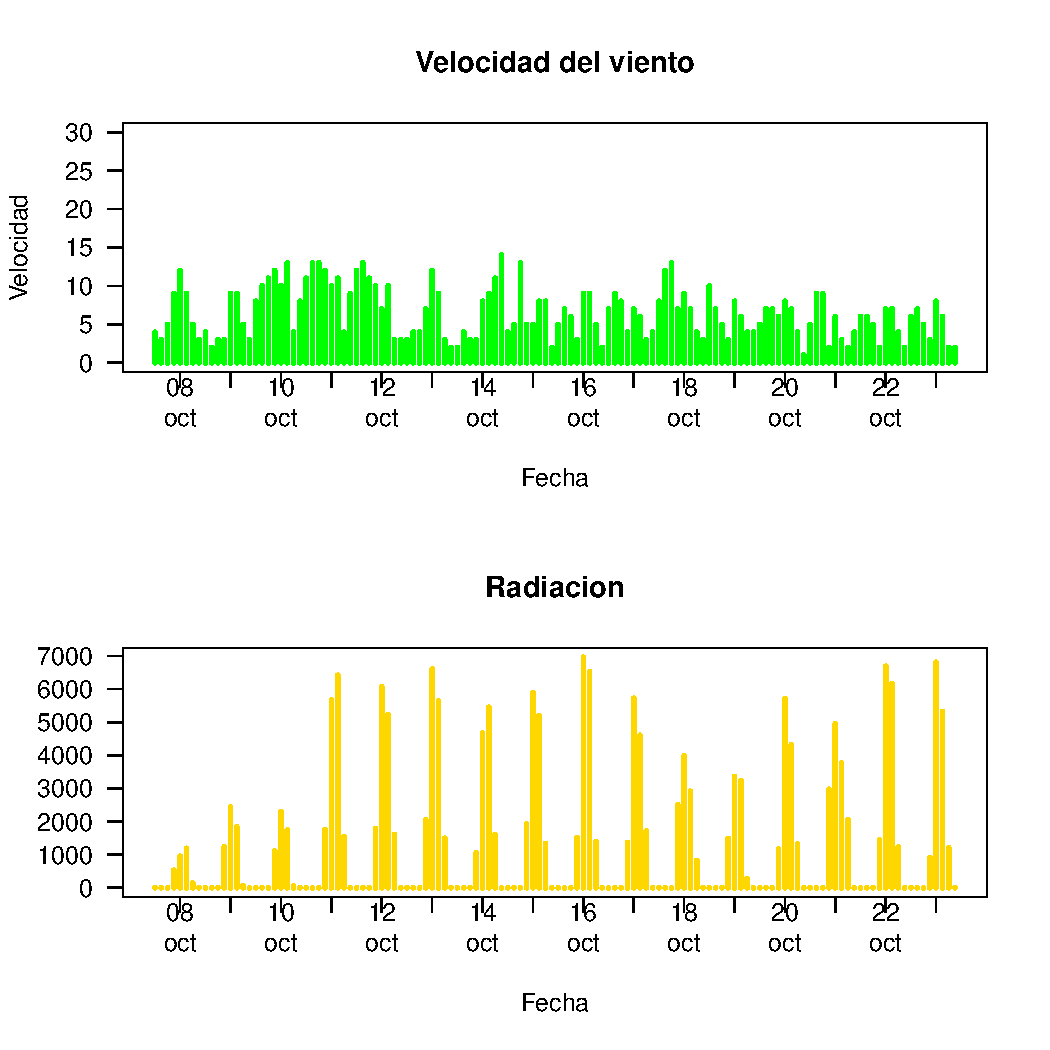
\includegraphics[width=\maxwidth]{figure/Figwind-1} 

\end{knitrout}
\end{figure}

\begin{figure}[h!]
\begin{knitrout}
\definecolor{shadecolor}{rgb}{0.969, 0.969, 0.969}\color{fgcolor}
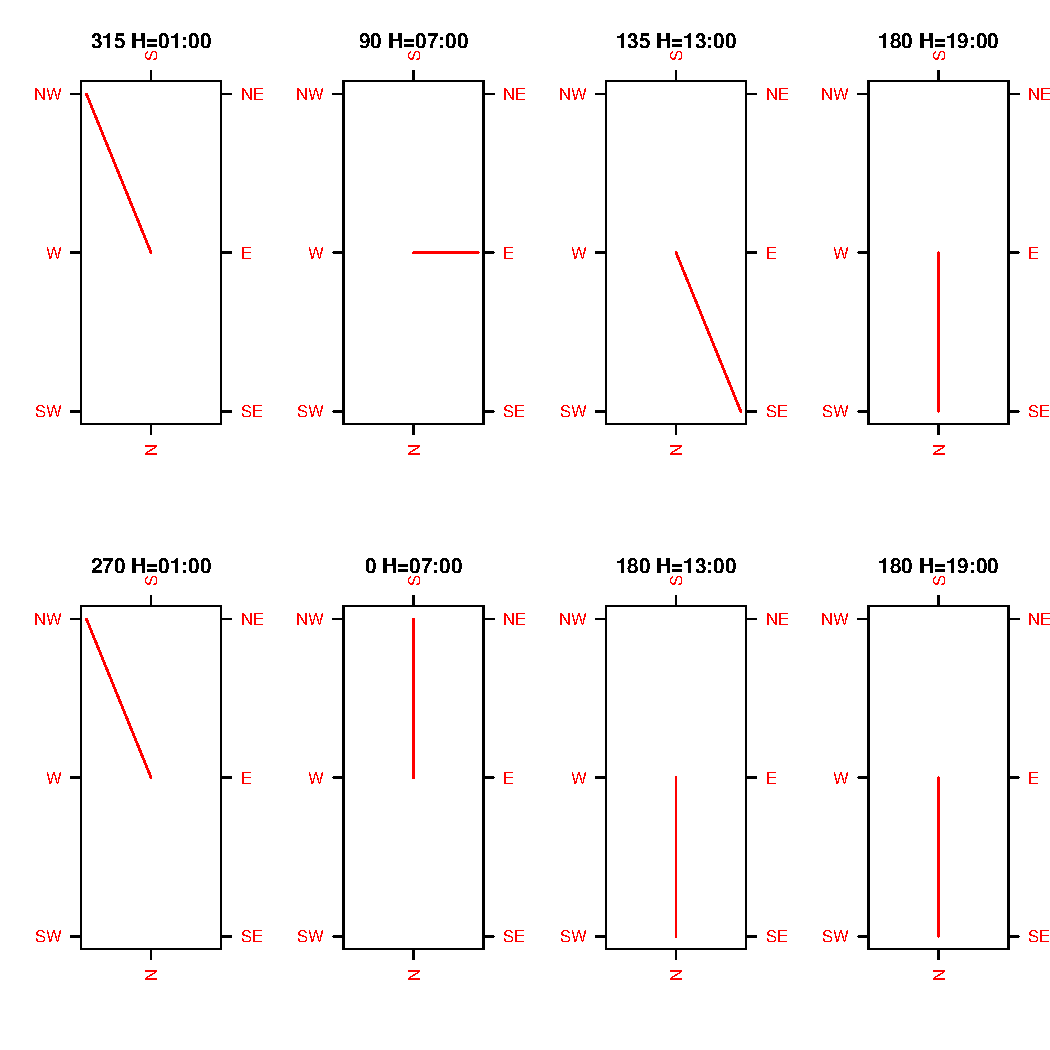
\includegraphics[width=\maxwidth]{figure/Figdir-1} 

\end{knitrout}
\end{figure}

\begin{figure}[h!]
\begin{knitrout}
\definecolor{shadecolor}{rgb}{0.969, 0.969, 0.969}\color{fgcolor}
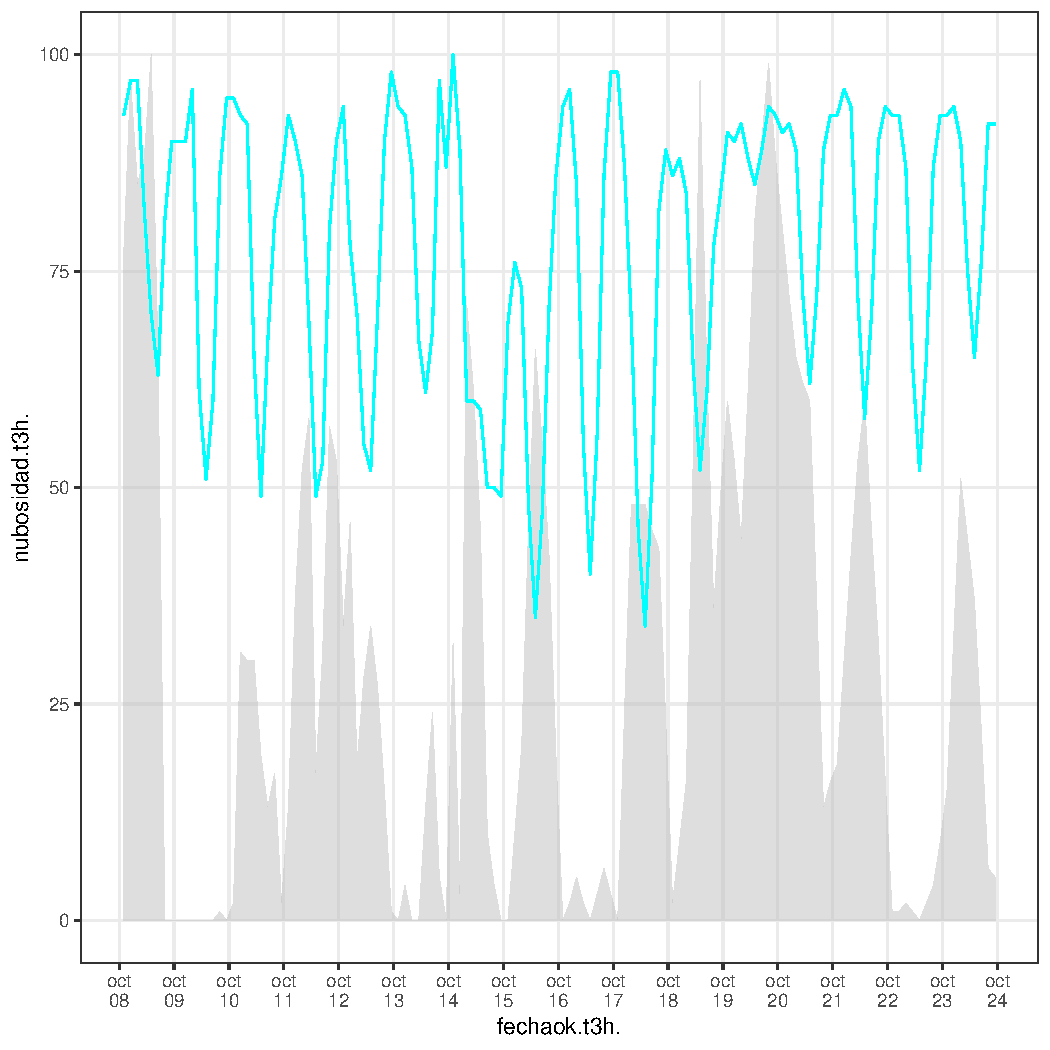
\includegraphics[width=\maxwidth]{figure/Fig1-1} 

\end{knitrout}
\end{figure}

\newpage

% latex table generated in R 3.3.3 by xtable 1.8-4 package
% Thu Oct 17 08:37:01 2019
\begin{tabular}{rllll}
  \hline
 & 1 & 2 & 3 & 4 \\ 
  \hline
1 & 20191008 02:00 & 1019 & 19.37 & 315 \\ 
  2 & 20191008 05:00 & 1019 & 19.4 & 45 \\ 
  3 & 20191008 08:00 & 1020 & 19.34 & 135 \\ 
  4 & 20191008 11:00 & 1021 & 21.05 & 135 \\ 
  5 & 20191008 14:00 & 1020 & 22.58 & 180 \\ 
  6 & 20191008 17:00 & 1019 & 22.92 & 180 \\ 
  7 & 20191008 20:00 & 1018 & 19.19 & 180 \\ 
  8 & 20191008 23:00 & 1019 & 17.63 & 270 \\ 
  9 & 20191009 02:00 & 1018 & 17.17 & 270 \\ 
  10 & 20191009 05:00 & 1017 & 17.33 & 315 \\ 
  11 & 20191009 08:00 & 1017 & 15.78 & 0 \\ 
  12 & 20191009 11:00 & 1018 & 21.91 & 180 \\ 
  13 & 20191009 14:00 & 1017 & 25.16 & 180 \\ 
  14 & 20191009 17:00 & 1016 & 24.06 & 180 \\ 
  15 & 20191009 20:00 & 1016 & 19.41 & 180 \\ 
  16 & 20191009 23:00 & 1018 & 17.87 & 0 \\ 
  17 & 20191010 02:00 & 1019 & 17.26 & 0 \\ 
  18 & 20191010 05:00 & 1019 & 17.23 & 0 \\ 
  19 & 20191010 08:00 & 1020 & 17.52 & 0 \\ 
  20 & 20191010 11:00 & 1022 & 21.85 & 45 \\ 
  21 & 20191010 14:00 & 1021 & 25.45 & 90 \\ 
  22 & 20191010 17:00 & 1020 & 23.02 & 135 \\ 
  23 & 20191010 20:00 & 1021 & 20.22 & 180 \\ 
  24 & 20191010 23:00 & 1022 & 18.28 & 0 \\ 
  25 & 20191011 02:00 & 1022 & 17.33 & 0 \\ 
  26 & 20191011 05:00 & 1021 & 17.49 & 0 \\ 
  27 & 20191011 08:00 & 1021 & 17.5 & 0 \\ 
  28 & 20191011 11:00 & 1022 & 21.67 & 45 \\ 
  29 & 20191011 14:00 & 1021 & 25.63 & 45 \\ 
  30 & 20191011 17:00 & 1019 & 25.62 & 135 \\ 
  31 & 20191011 20:00 & 1019 & 21.41 & 180 \\ 
  32 & 20191011 23:00 & 1020 & 19.11 & 0 \\ 
  33 & 20191012 02:00 & 1019 & 18.02 & 0 \\ 
  34 & 20191012 05:00 & 1017 & 18.08 & 0 \\ 
  35 & 20191012 08:00 & 1017 & 17.46 & 0 \\ 
  36 & 20191012 11:00 & 1019 & 22.53 & 45 \\ 
  37 & 20191012 14:00 & 1017 & 25.94 & 135 \\ 
  38 & 20191012 17:00 & 1015 & 24.3 & 135 \\ 
  39 & 20191012 20:00 & 1016 & 20.93 & 180 \\ 
  40 & 20191012 23:00 & 1017 & 18.67 & 315 \\ 
  41 & 20191013 02:00 & 1017 & 18.12 & 0 \\ 
  42 & 20191013 05:00 & 1016 & 17.4 & 315 \\ 
  43 & 20191013 08:00 & 1017 & 18.07 & 270 \\ 
  44 & 20191013 11:00 & 1018 & 22.91 & 180 \\ 
  45 & 20191013 14:00 & 1017 & 24.78 & 180 \\ 
  46 & 20191013 17:00 & 1015 & 23.91 & 180 \\ 
  47 & 20191013 20:00 & 1015 & 19.72 & 180 \\ 
  48 & 20191013 23:00 & 1015 & 19.9 & 315 \\ 
  49 & 20191014 02:00 & 1016 & 17.17 & 315 \\ 
  50 & 20191014 05:00 & 1014 & 16.87 & 0 \\ 
  51 & 20191014 08:00 & 1013 & 20.48 & 135 \\ 
  52 & 20191014 11:00 & 1015 & 22.23 & 135 \\ 
  53 & 20191014 14:00 & 1014 & 24.09 & 135 \\ 
  54 & 20191014 17:00 & 1011 & 25.42 & 135 \\ 
  55 & 20191014 20:00 & 1012 & 23.13 & 315 \\ 
  56 & 20191014 23:00 & 1015 & 19.66 & 315 \\ 
  57 & 20191015 02:00 & 1017 & 16.88 & 135 \\ 
  58 & 20191015 05:00 & 1018 & 14.69 & 0 \\ 
  59 & 20191015 08:00 & 1019 & 14.36 & 0 \\ 
  60 & 20191015 11:00 & 1019 & 18.86 & 0 \\ 
  61 & 20191015 14:00 & 1019 & 22.99 & 135 \\ 
  62 & 20191015 17:00 & 1019 & 21.02 & 180 \\ 
  63 & 20191015 20:00 & 1020 & 17.46 & 180 \\ 
  64 & 20191015 23:00 & 1021 & 15.1 & 225 \\ 
  65 & 20191016 02:00 & 1022 & 13.36 & 0 \\ 
  66 & 20191016 05:00 & 1022 & 12.21 & 0 \\ 
  67 & 20191016 08:00 & 1022 & 12.73 & 0 \\ 
  68 & 20191016 11:00 & 1022 & 17.61 & 135 \\ 
  69 & 20191016 14:00 & 1022 & 21.95 & 135 \\ 
  70 & 20191016 17:00 & 1021 & 20.25 & 180 \\ 
  71 & 20191016 20:00 & 1021 & 16.95 & 180 \\ 
  72 & 20191016 23:00 & 1020 & 14.92 & 315 \\ 
  73 & 20191017 02:00 & 1020 & 13.48 & 0 \\ 
  74 & 20191017 05:00 & 1020 & 12.55 & 0 \\ 
  75 & 20191017 08:00 & 1020 & 13.21 & 0 \\ 
  76 & 20191017 11:00 & 1020 & 18.13 & 45 \\ 
  77 & 20191017 14:00 & 1020 & 22.48 & 90 \\ 
  78 & 20191017 17:00 & 1020 & 20.74 & 135 \\ 
  79 & 20191017 20:00 & 1021 & 17.53 & 90 \\ 
  80 & 20191017 23:00 & 1021 & 15.96 & 0 \\ 
  81 & 20191018 02:00 & 1021 & 14.96 & 0 \\ 
  82 & 20191018 05:00 & 1021 & 14.15 & 0 \\ 
  83 & 20191018 08:00 & 1021 & 14.59 & 0 \\ 
  84 & 20191018 11:00 & 1021 & 18.56 & 45 \\ 
  85 & 20191018 14:00 & 1021 & 22.08 & 90 \\ 
  86 & 20191018 17:00 & 1021 & 20.76 & 135 \\ 
  87 & 20191018 20:00 & 1020 & 18.13 & 180 \\ 
  88 & 20191018 23:00 & 1021 & 16.63 & 0 \\ 
  89 & 20191019 02:00 & 1021 & 15.14 & 0 \\ 
  90 & 20191019 05:00 & 1020 & 15.14 & 315 \\ 
  91 & 20191019 08:00 & 1019 & 15.11 & 315 \\ 
  92 & 20191019 11:00 & 1019 & 16.63 & 45 \\ 
  93 & 20191019 14:00 & 1020 & 18.15 & 90 \\ 
  94 & 20191019 17:00 & 1020 & 17.48 & 90 \\ 
  95 & 20191019 20:00 & 1020 & 16.37 & 45 \\ 
  96 & 20191019 23:00 & 1020 & 16.05 & 0 \\ 
  97 & 20191020 02:00 & 1020 & 15.88 & 0 \\ 
  98 & 20191020 05:00 & 1020 & 15.27 & 0 \\ 
  99 & 20191020 08:00 & 1020 & 15.32 & 0 \\ 
  100 & 20191020 11:00 & 1021 & 17.91 & 45 \\ 
  101 & 20191020 14:00 & 1021 & 20.1 & 90 \\ 
  102 & 20191020 17:00 & 1021 & 18.66 & 90 \\ 
  103 & 20191020 20:00 & 1020 & 16.37 & 135 \\ 
  104 & 20191020 23:00 & 1021 & 15.26 & 0 \\ 
  105 & 20191021 02:00 & 1021 & 14.29 & 315 \\ 
  106 & 20191021 05:00 & 1021 & 12.25 & 315 \\ 
  107 & 20191021 08:00 & 1020 & 11.62 & 315 \\ 
  108 & 20191021 11:00 & 1021 & 16.37 & 0 \\ 
  109 & 20191021 14:00 & 1022 & 20.82 & 135 \\ 
  110 & 20191021 17:00 & 1021 & 19.12 & 90 \\ 
  111 & 20191021 20:00 & 1021 & 15.81 & 0 \\ 
  112 & 20191021 23:00 & 1022 & 13.8 & 315 \\ 
  113 & 20191022 02:00 & 1022 & 12.16 & 315 \\ 
  114 & 20191022 05:00 & 1022 & 10.27 & 315 \\ 
  115 & 20191022 08:00 & 1022 & 10.14 & 315 \\ 
  116 & 20191022 11:00 & 1022 & 15.54 & 90 \\ 
  117 & 20191022 14:00 & 1023 & 20.62 & 135 \\ 
  118 & 20191022 17:00 & 1022 & 19.2 & 135 \\ 
  119 & 20191022 20:00 & 1021 & 16.08 & 135 \\ 
  120 & 20191022 23:00 & 1021 & 14.31 & 270 \\ 
  121 & 20191023 02:00 & 1021 & 12.97 & 315 \\ 
  122 & 20191023 05:00 & 1020 & 11.68 & 315 \\ 
  123 & 20191023 08:00 & 1019 & 11.85 & 315 \\ 
  124 & 20191023 11:00 & 1019 & 16.39 & 180 \\ 
  125 & 20191023 14:00 & 1019 & 20.53 & 180 \\ 
  126 & 20191023 17:00 & 1018 & 19.13 & 180 \\ 
  127 & 20191023 20:00 & 1017 & 16.21 & 180 \\ 
  128 & 20191023 23:00 & 1016 & 14.39 & 270 \\ 
   \hline
\end{tabular}



La temperaturea media es 8.5676823

La temperaturea maxima es 25.94

\end{document}
